\section{Tests}
Several tests have been included in our assignment to test the functionality of our implemented functions. Also, new ones have been created to further test the functionality of our fasto-compiler.\\
For example, we have written the following test for the functionality of the \textit{or}-operator, which looks as so:\\
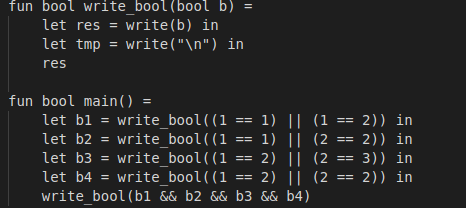
\includegraphics[width=\linewidth]{Materials/Tests/OrTest}
This test (alongside most others) suceed by matching expected input. In the case of the test above, the expected output, which it matches, looks like the following:\\
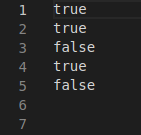
\includegraphics[width=0.4\linewidth]{Materials/Tests/OrExpected}\\
Some tests have been made only to test the typechecker.These tests purposefully use nonsensical types (like using the \textit{or}-operator between integers or multiplying an int with a bool). The typechecker-test with regards to the \textit{or}-operator looks like so:\\
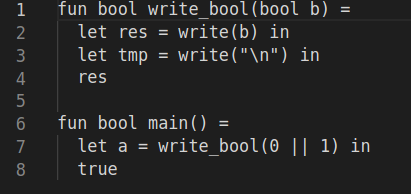
\includegraphics[width=\linewidth]{Materials/Tests/OrTypeCheck}\\
The test succeeds as the accompanying \textit{.err}-file expects the appropriate error-message reflecting the error. In this case, the error is a type-missmatch, as the \textit{or}-operator expects two bools but is given two integers instead. Also, this test doubles as a reassurence that $0$ and $1$ aren't evaluated as \textit{false} and \textit{true}, respectively. 
